\documentclass[14pt]{extreport}
\usepackage{gost}

\begin{document}

\pagestyle{empty}
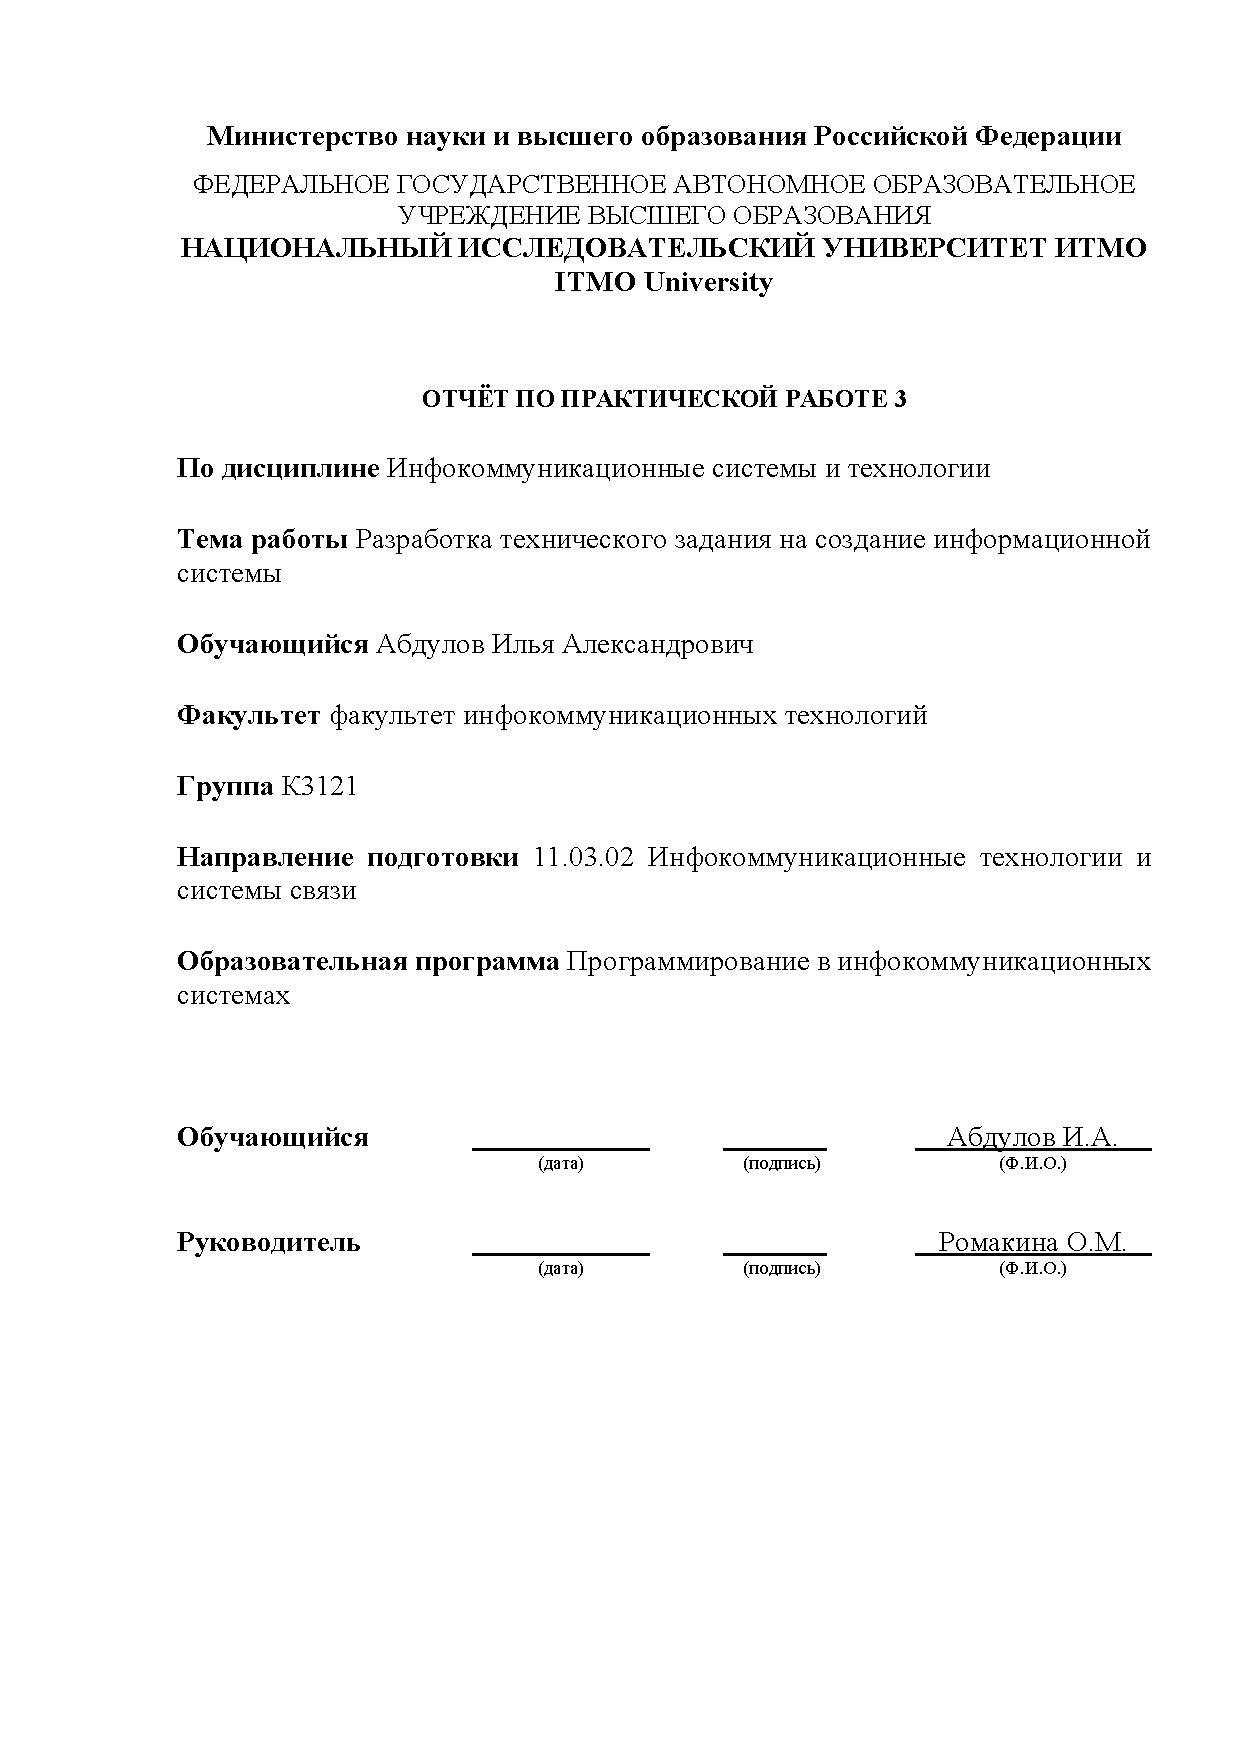
\includepdf{titulCourse.pdf}
\pagestyle{plain}

\tableofcontents

\intro

Практическая работа 6 является актуальной, потому что является описанием основных функциональных элементов будущего мобильного приложения. Приложение Better Row представляет из себя приложение, куда пользователь заносит данные своих тренировок, чтобы приложение показывало и сохраняло текущие показатели и прогресс. Использование приложения придаст тренировкам осознанности, что поможет в достижении лучшего результата.

Целью данной работы является описание предметной области функционирования и построение функциональной модели в стандарте IDEF0, которая включает 3 уровня декомпозиции. Необходимо предусмотреть обратные связи между работами по входу или управлению. В процессе работы будет использован инструмент для построения IDEF0 моделей – Ramus.

\chapter{Основная часть}

\section{Предметная область функционирования}

Приложение предназначено для развития спортивной деятельности в университете ИТМО, информационная система разрабатывается для клуба по академической гребли. Приложение позволяет сохранять данные о тренировке и всесторонне анализировать их для удобства отслеживания прогресса.

\section{Методология IDEF0}

\begin{figure}[H]
\centerline{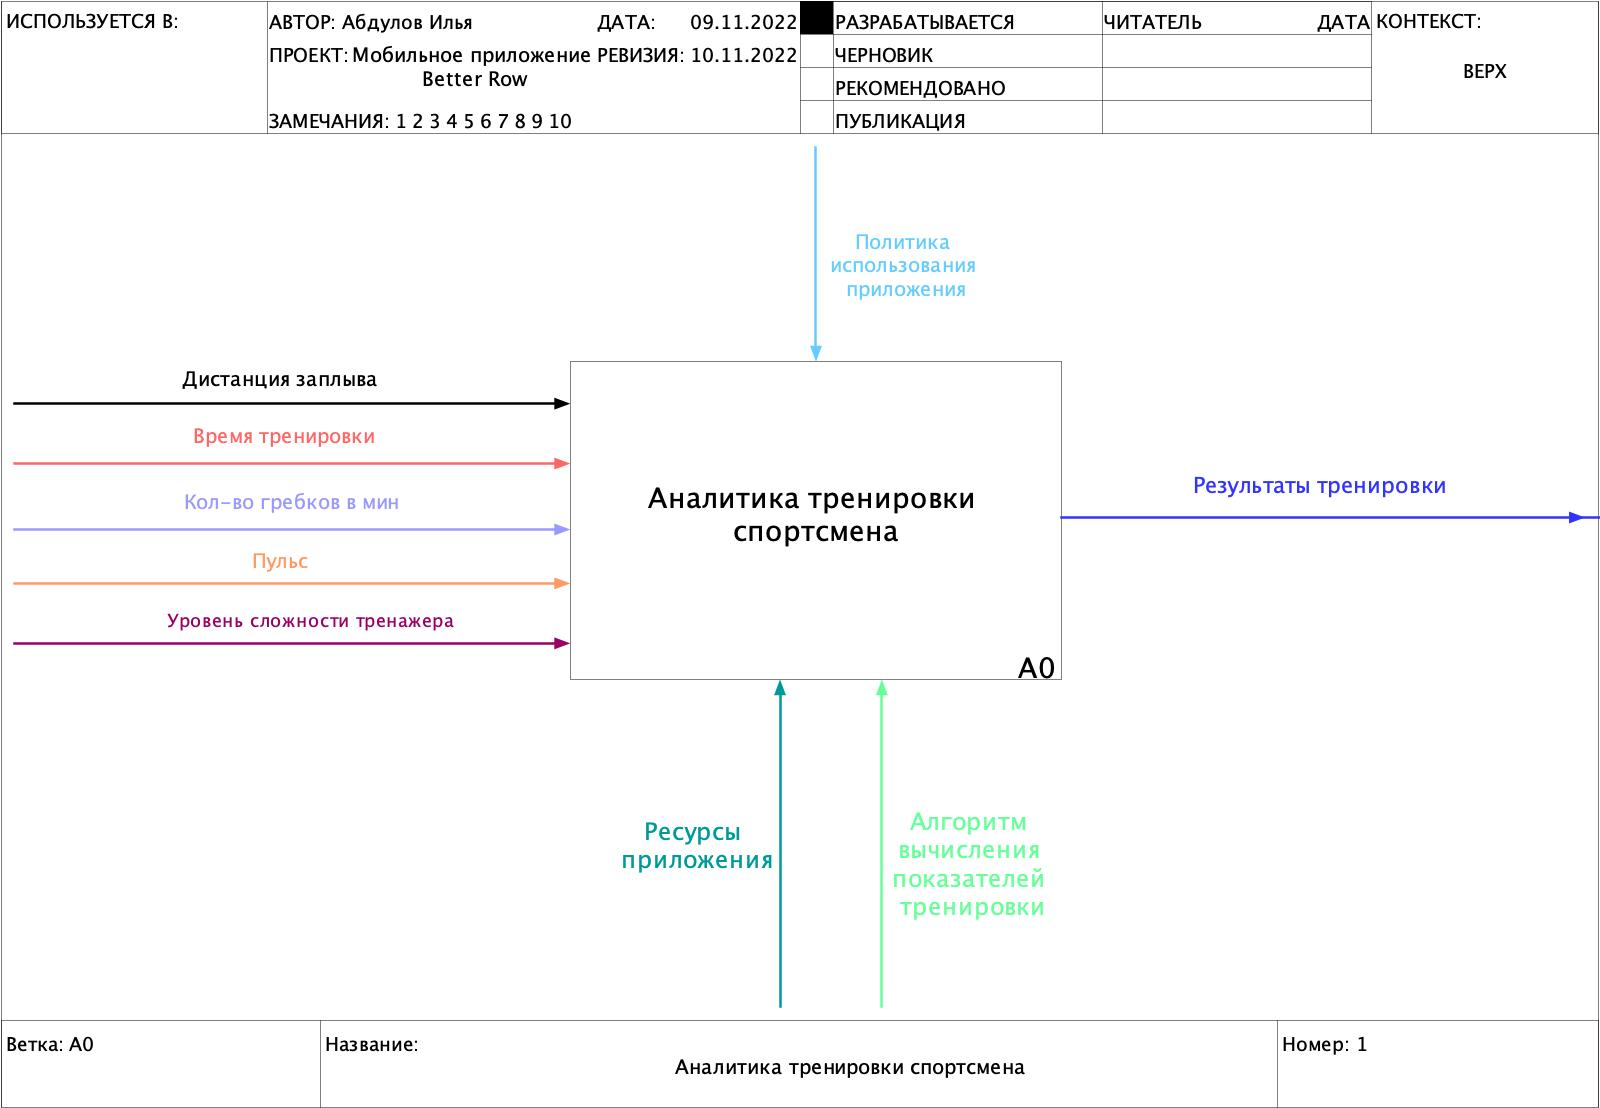
\includegraphics[width=1\linewidth]{01_A0.jpg}}
\caption{Функциональная модель в стандарте IDEF0}
\label{fig11}
\end{figure}

\begin{figure}[H]
\centerline{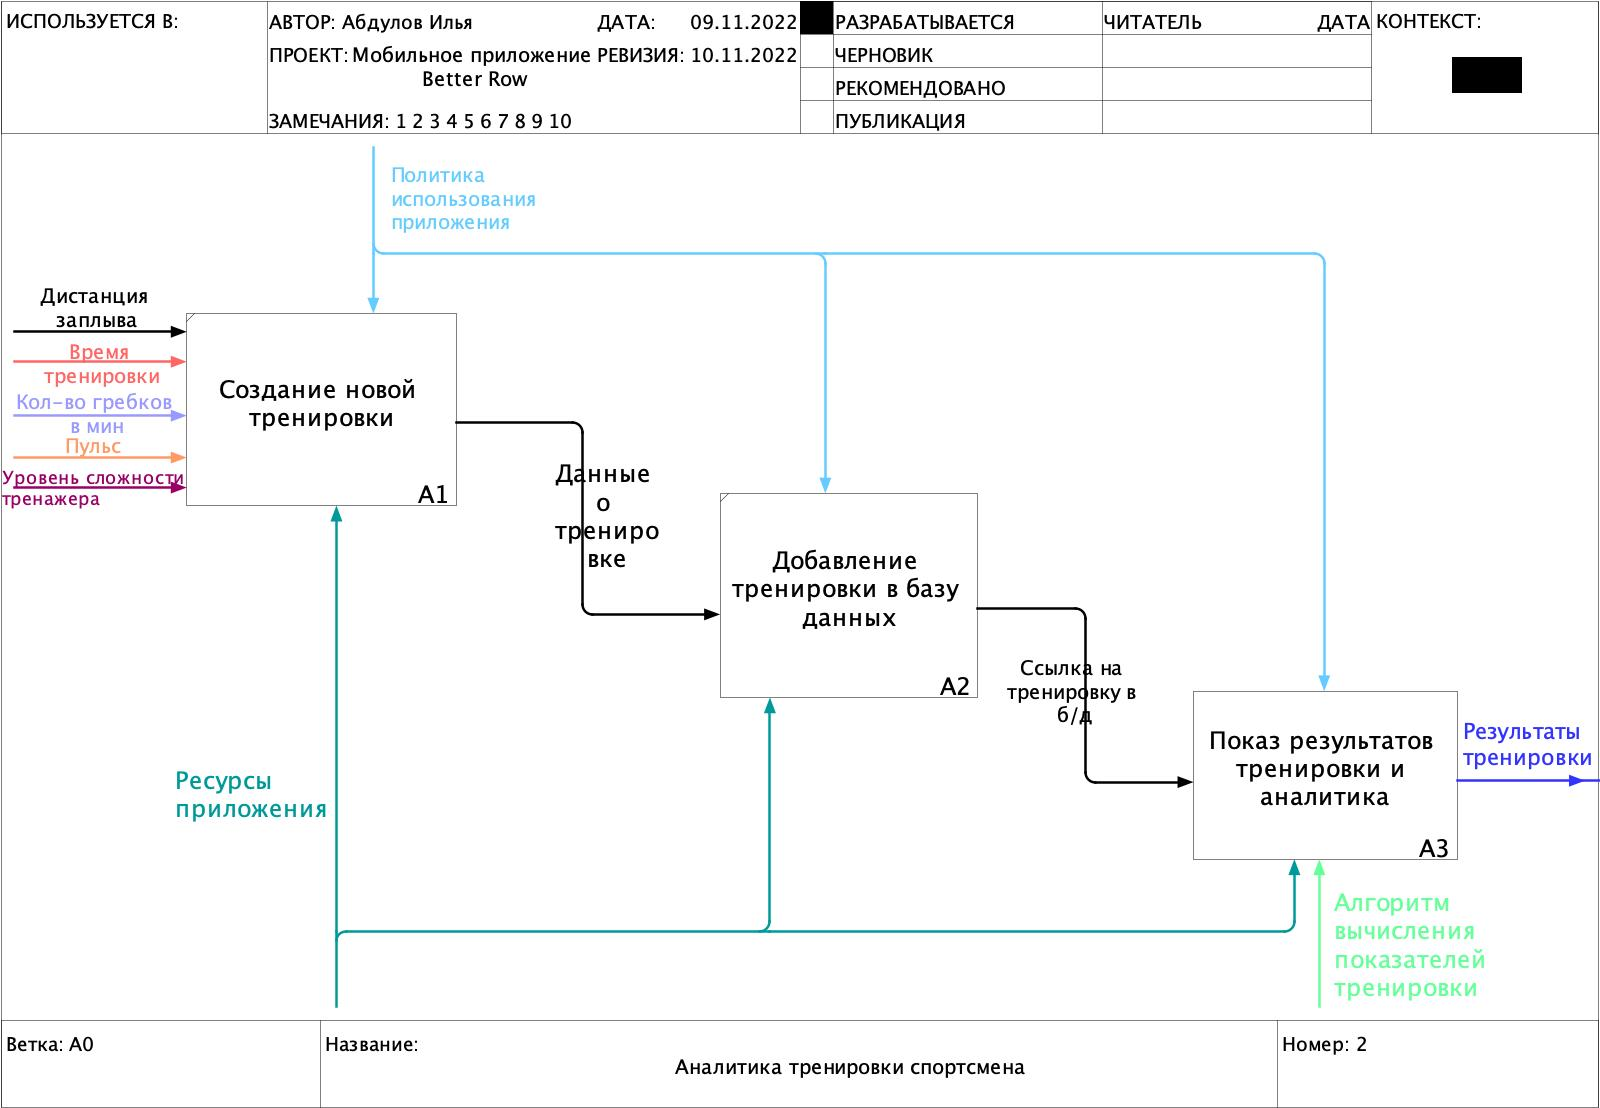
\includegraphics[width=1\linewidth]{02_A0.jpg}}
\caption{Первый уровень декомпозиции "Аналитика тренировки спортсмена"}
\label{fig12}
\end{figure}

\begin{figure}[H]
\centerline{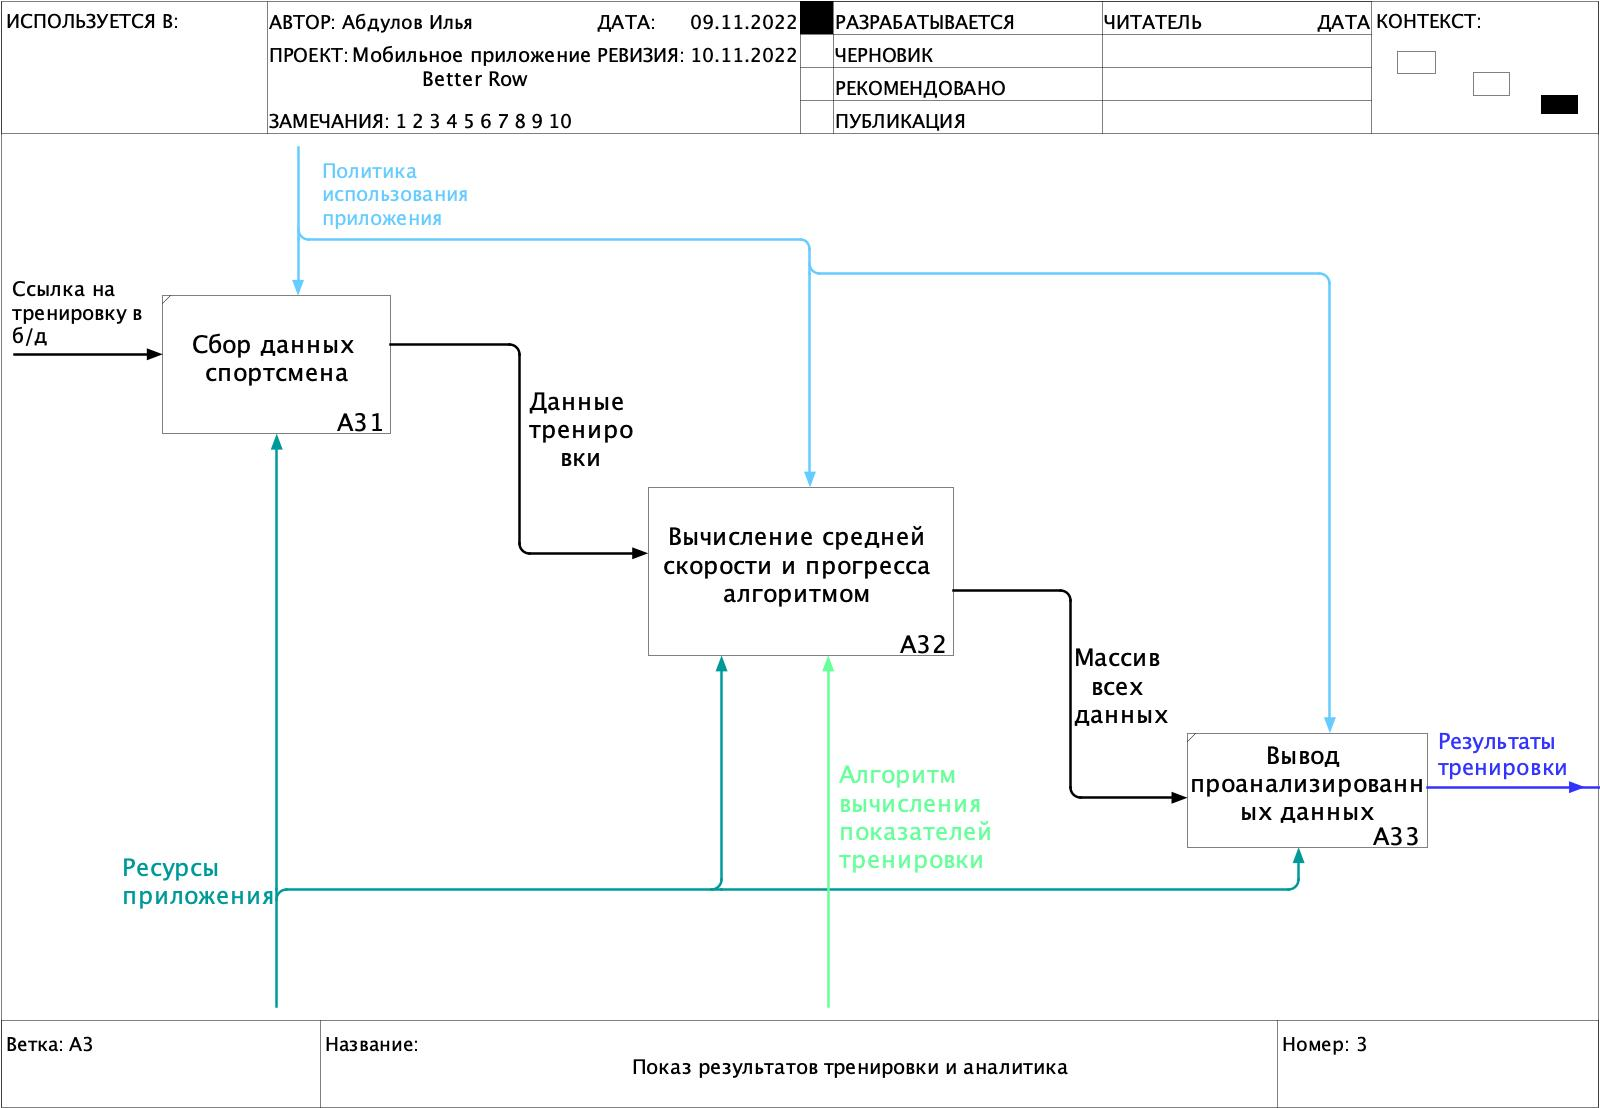
\includegraphics[width=1\linewidth]{03_A3.jpg}}
\caption{Второй уровень декомпозиции "Показ результатов тренировки и аналитика"}
\label{fig13}
\end{figure}

\begin{figure}[H]
\centerline{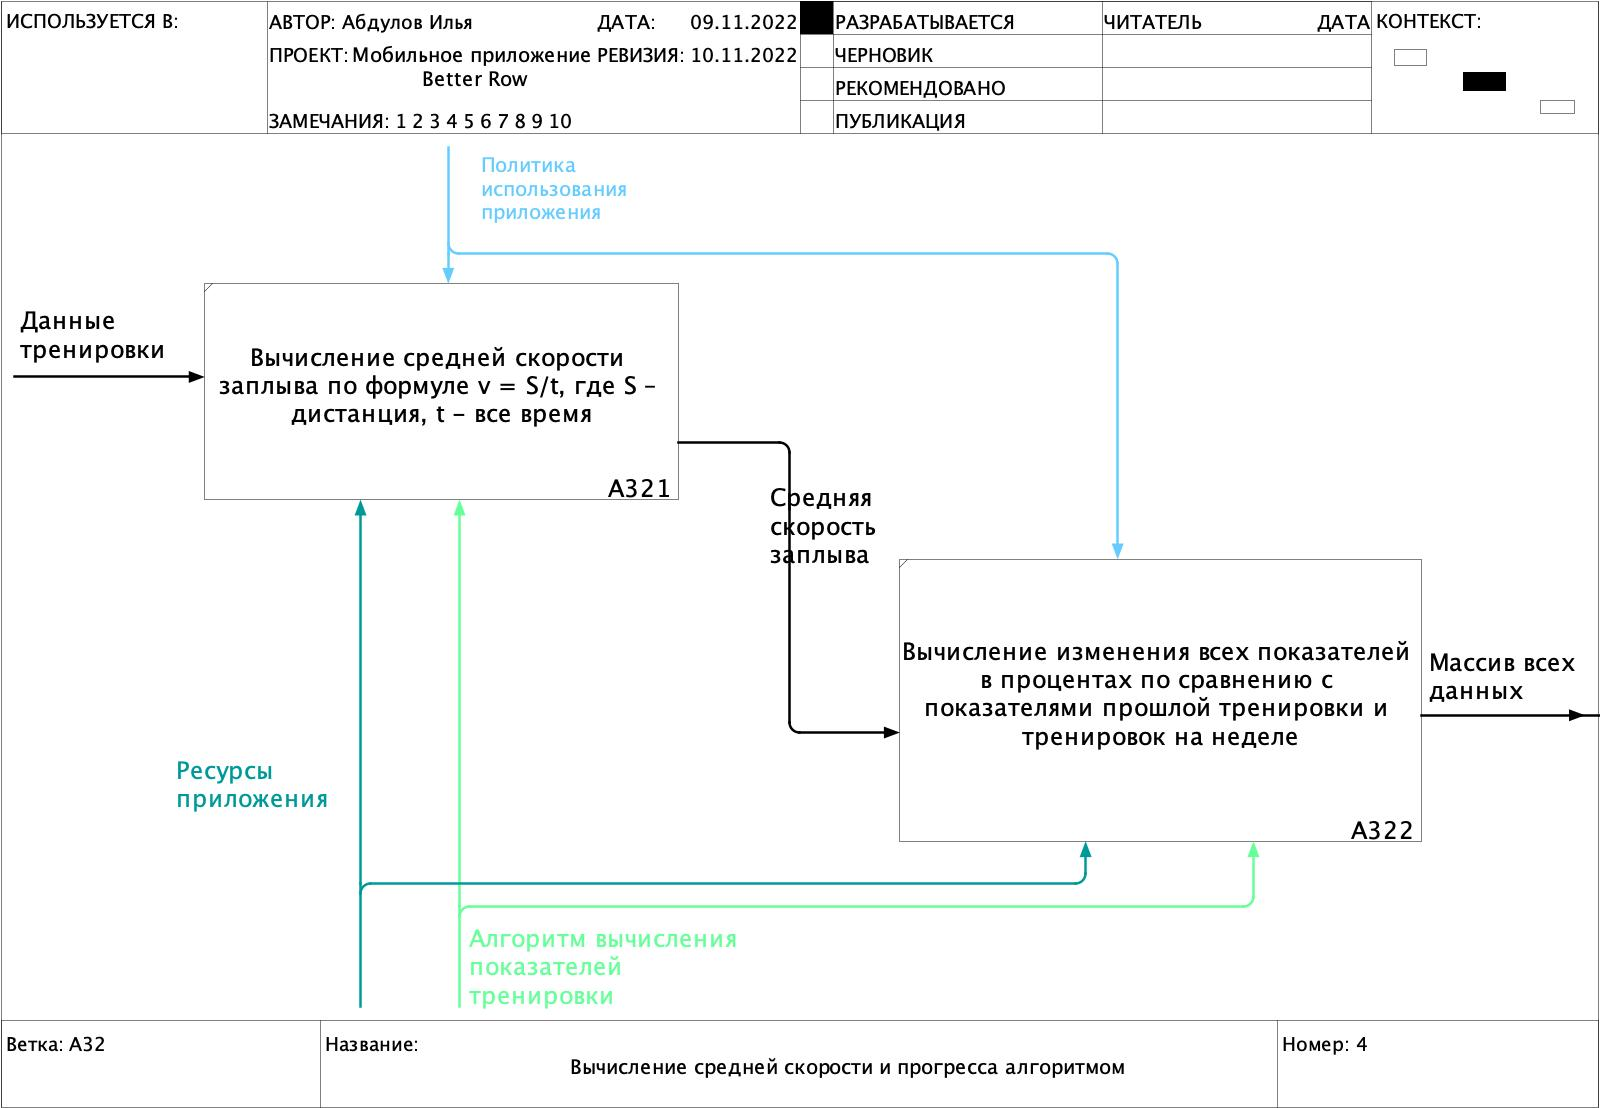
\includegraphics[width=1\linewidth]{04_A32.jpg}}
\caption{Третий уровень декомпозиции "Вычисление средней скорости и прогресса алгоритмом"}
\label{fig14}
\end{figure}

Предусмотрено наличие обратных связей между работами по входу или управлению. В функциональной модели и декомпозициях обратных связей нет.

\conclusions

Цель работы была достигнута. Была описана предметная область функционирования. В отчёте были представлены построенные функциональные модели IDEF0, которые содержат 3 уровня декомпозиции. Предусмотрены обратные связи между работами по входу или управлению.

\newpage
\begin{thebibliography}{99}

\bibitem{bib1}Приложение Ramus для построения IDEF0 моделей — URL: \url{http://ramussoftware.com/} (дата обращения 09.11.2022).	

\bibitem{bib2}Интернет-статья по методологии IDEF0 — URL: \url{https://trinion.org/blog/idef0-znakomstvo-s-notaciey-i-primer-ispolzovaniya} (дата обращения 09.11.2022).	
	
\end{thebibliography}

\end{document}
